\documentclass[10pt,a4paper]{article}
\usepackage[margin=18mm]{geometry}
\usepackage{amsmath,booktabs,graphicx,hyperref}
\title{Ion CSA v3 response study}
\date{\today}
\begin{document}\maketitle
The study processes 8,000 event IDs per sample at 4 mm pitch
and 40 ms frame width. Every pixel with charge retains its
complete event history, including empty frames, two quiet leading frames and a
three-second recovery window. There is no S/N cut. Signed reconstructed counts,
including negative noise fluctuations, are retained.

The circuit is the provisional v3 design, nominal 20 s discharge, with 5 ms
centred voltage averages, 1.25 pF external capacitance and 3 fF feedback. The input
uses uniform mean collection within each frame and the established central
0.5 mm square-pad weighting benchmark in an infinite grounded plane. The pad
weighting potential is one, with zero on the surrounding plane and at infinity,
in homogeneous dielectric. The ion speed is 3 m/s through the finite 5 mm gap.
The charge integral is $e[1-\phi_w(g)]$ per collected ion.

\begin{center}\small\begin{tabular}{lrrrr}\toprule Sample & ENC before & ENC after & Bias before (\%) & Bias after (\%)\\\midrule
Double beta & 58.44 & 58.95 & +2.597 & -0.621 \\\bottomrule\end{tabular}\end{center}

The same transistor circuit was recalibrated at 20, 30 and 40 ms. Noise uses its
one-sided stationary operating-point spectrum from 0.0001 Hz to 1 MHz, filtered
by the 5 ms average and the decay-corrected frame difference. Gaussian samples
retain temporal covariance; pad channels are independent. This stationary noise
approximation is also applied to compressed mean signals.
\begin{center}\begin{tabular}{rrrrr}\toprule
Frame (ms) & Fitted $\tau$ (s) & Filtered gain ($\mu$V/ion) & ENC (ions RMS) & Lag-1 correlation\\\midrule
20 & 19.5441 & 40.157 & 51.26 & -0.3292 \\
40 & 19.5440 & 41.479 & 58.95 & -0.2738 \\
\bottomrule\end{tabular}\end{center}

S/N is the noiseless recovered signal divided by frame ENC, evaluated over all
positive input pixel--frame cells. The cell-weighted and event-weighted means
are shown separately. Compression compares the noiseless transistor response
with the calibrated linear prediction; the flags require a deficit of at least
one frame ENC. A pad history is counted once per event if any positive-input
bucket passes the indicated local-loss criterion.

\begin{center}\scriptsize\begin{tabular}{lrrrrrrr}\toprule
Sample & Events & ENC & Mean S/N & Event mean S/N & Loss50 events (\%) & Deficit (\%) & Total bias (\%)\\\midrule
Double beta & 8000 & 58.95 & 5.347 & 6.183 & 9.09 & 0.620 & -0.621 \\
\bottomrule\end{tabular}\end{center}

The positive-cell compression deficit is
$\sum_{N_n>0}\max(\widehat N_{\rm linear,n}-\widehat N_{\rm CSA,n},0)/\sum N_n$.
The signed total bias is $(\sum\widehat N_{\rm CSA,n}-\sum N_n)/\sum N_n$,
including quiet frames and recovery. The linear prediction's own calibration
bias is saved separately, as is the noisy summed estimate. The corrected reconstruction solves $M\widehat{\mathbf N}=\mathbf y$ using the saved three-frame response. The same banded solve is applied to the noiseless signal and the existing noise realisation. Its covariance is $M^{-1}C_yM^{-T}$. Quiet boundary frames are retained, and exact history-dependent frame variances enter S/N. This removes the linear normalization bias and temporal mixing while preserving the circuit compression.

\begin{figure}[ht]\centering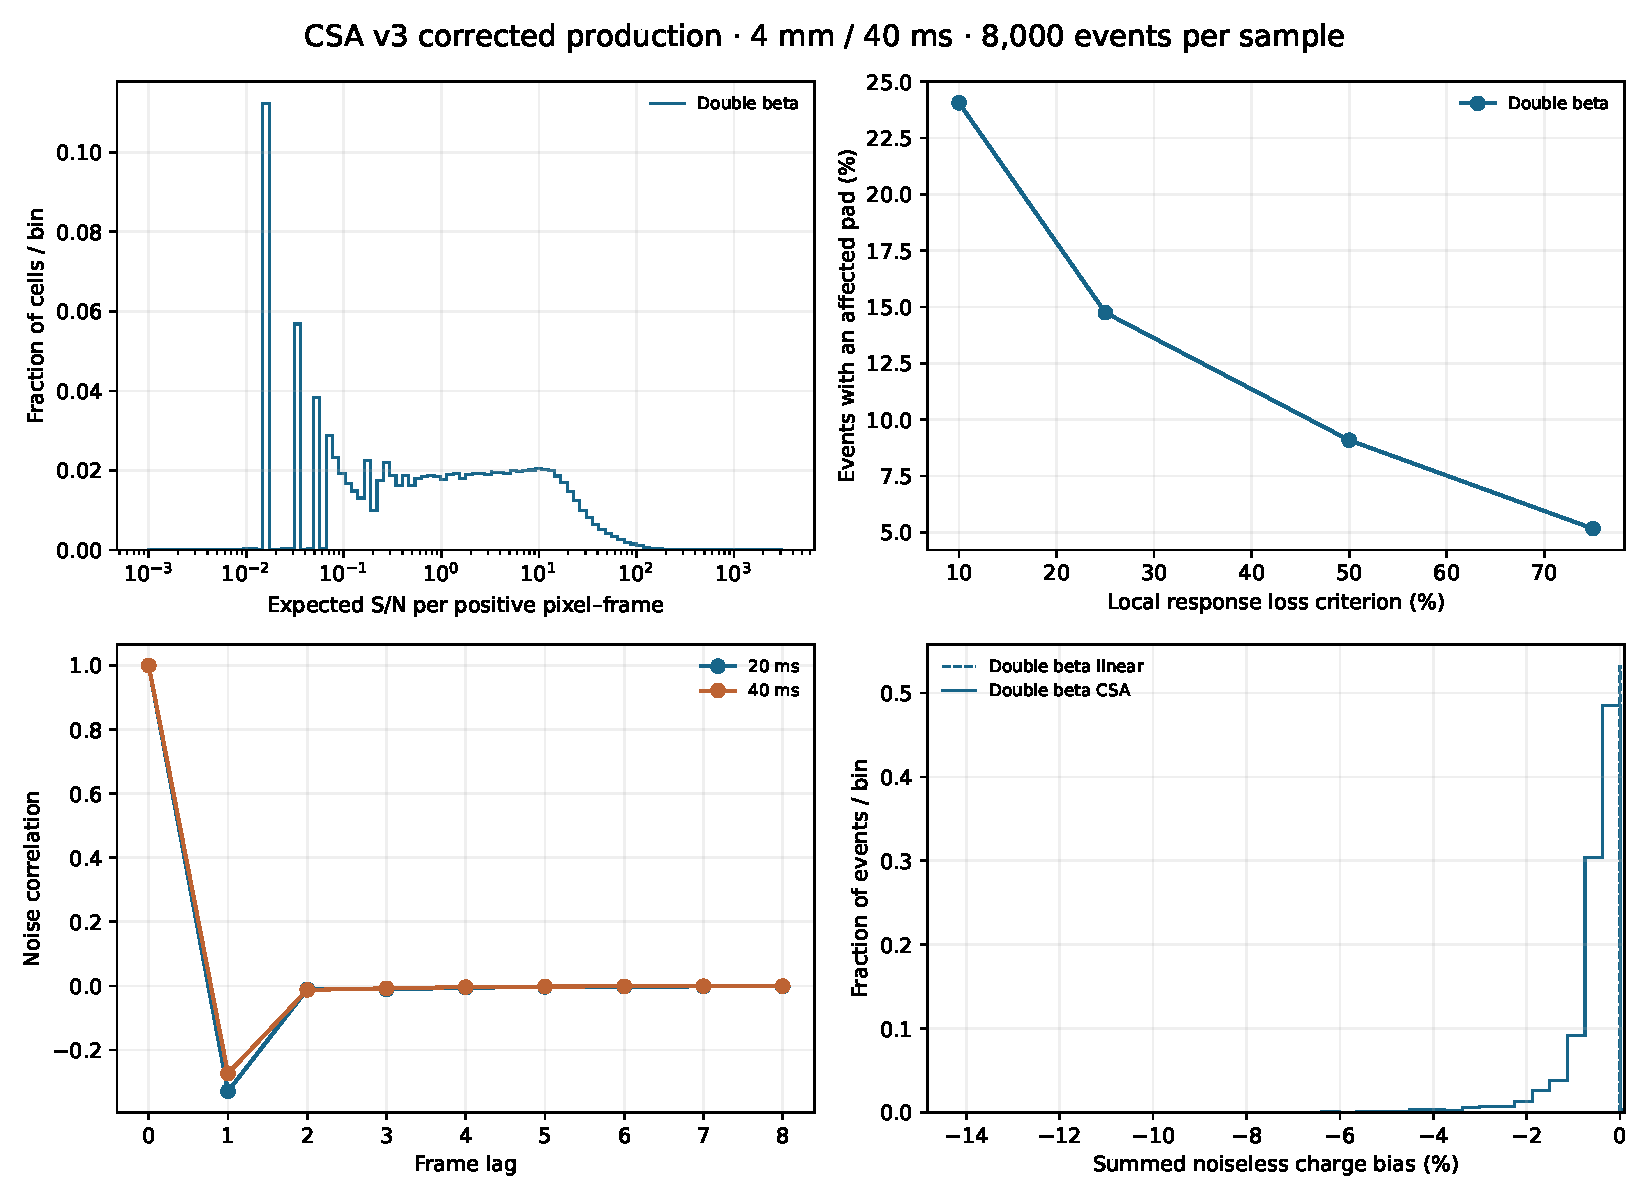
\includegraphics[width=\linewidth]{diagnostics.pdf}
\caption{Saved study quality, compression, covariance and charge-bias diagnostics.
Dashed charge-bias curves use the linear estimator; solid curves include
transistor response where directly simulated.}
\end{figure}

The inherited fast response is checked against control histories spanning predicted
output voltage. The inherited voltage range keeps remaining transformed control errors
below the configured 0.5 ENC. The final voltage guard is 0.63 V and the
largest remaining control error is 0.3914 ENC. Independent solver refinement
changes the sampled response by at most 1.916e-05 ENC. Independent checks cover
finite-path charge, spectral integration, covariance convergence and positive
definiteness, sampled zero-input mean/variance/covariance, input ion ledgers and
Float32 storage errors relative to Float64 calculations.

Response files use \texttt{nausicaa.ion\_csa\_response.pilot.v2}. Each saves the
selected IDs, parent file/hash, exact cards, code identity, stable per-pad seed,
frame covariance, input counts, mean voltages, linear/noiseless/noisy recovered
ions and compression flags. Files are written atomically and marked complete
after the requested event ledgers pass.

The companion \texttt{ion\_csa.html} provides sample and compression-severity
selectors, diagnostic distributions and typical/weak/compressed pad histories.
S/N is a quality observable; final analysis determines acceptable performance.
Spatial noise occupancy requires a finite readout area; the present controls
use zero-input histories on the selected channels.

From the repository root:
\begin{verbatim}
work/event-viewer-venv/bin/python scripts/production/run_ion_csa_correction.py
# Presentation only:
work/event-viewer-venv/bin/python scripts/production/present_ion_csa_pilot.py \
  --results RESULTS_DIRECTORY
\end{verbatim}
\end{document}
